\documentclass[11pt,a4paper]{article}
\usepackage[utf8]{inputenc}
\usepackage[T1]{fontenc}
\usepackage{lmodern}
\usepackage[english]{babel}
\usepackage{microtype}
\usepackage[a4paper,margin=2.4cm]{geometry}
\usepackage{amsmath,amssymb}
\usepackage{graphicx}
\usepackage{booktabs}
\usepackage{xcolor}
\usepackage{float}
\usepackage{enumitem}
\usepackage[hidelinks]{hyperref}
\definecolor{accent}{HTML}{1F4E79}
\setlist{itemsep=2pt,topsep=3pt}
\graphicspath{{../figures/}}
\title{\color{accent}\bfseries From data to robust surgery schedules:\\[2pt]
\large learning the uncertainty of surgery duration and measuring its effect on operating-room plans}
\author{Deo Gratias Loutou\\[2pt]\small Master's student in computer science, Université de Haute-Alsace, Mulhouse\\
\small \href{https://github.com/LDGKM/surgery-duration-uncertainty}{github.com/LDGKM/surgery-duration-uncertainty}}
\date{October 2026}

\begin{document}
\maketitle

\begin{abstract}
Operating-room schedules are built on predicted surgery durations, yet the uncertainty around these predictions
is usually ignored or replaced by a uniform safety buffer. Using 6{,}385 operations from the open VitalDB dataset, we
(i) predict the time a patient occupies the operating room from information available before surgery,
(ii) build 80\% prediction intervals with five methods, including split conformal prediction and conformalized
quantile regression (CQR), and (iii) feed the learned uncertainty into a mixed-integer daily scheduling model whose
plans are then evaluated with the real durations. Gradient boosting reduces the mean absolute error from 50.7 to
45.6 minutes compared with per-procedure historical medians. Historical percentiles and raw quantile regression
under-cover (76.5\% and 67.7\% instead of 80\%), whereas CQR is calibrated (80.1\%) and has the lowest interval score
in all ten random splits. Coverage is not uniform across surgical contexts, which a per-department calibration only
partly fixes. In 200 simulated days, planning each case at its learned 80th percentile reduces overtime from 113
minutes per room and day (historical medians) to 19 minutes while keeping 88.7\% utilisation, 2.1 points more than a
uniform 15\% buffer with the same overtime. A budgeted robust model built on the learned deviations was markedly more
conservative. All code and results are public and reproducible.
\end{abstract}

\section{Introduction}
Operating rooms are among the most expensive hospital resources, and surgery durations are hard to predict: the same
procedure can take one hour or three. A schedule that ignores this variability causes overtime and cancellations; one
that over-protects leaves rooms idle \cite{cardoen2010,shehadeh2022}. Robust and distributionally robust scheduling
models address the problem, but they are only as good as their description of uncertainty
\cite{bertsimas2018}. This study asks two questions on open data:
\begin{enumerate}
  \item How well can the uncertainty of surgery duration be learned from pre-operative information, and does a
        stated 80\% interval really contain 80\% of cases, overall and within each surgical context?
  \item Does using that learned uncertainty in a scheduling model improve the overtime--utilisation trade-off,
        compared with classical assumptions (historical means, fixed buffers)?
\end{enumerate}
Machine learning for surgical time prediction is well studied \cite{martinez2021}; the contribution here is modest
and practical: an end-to-end, reproducible pipeline that evaluates the \emph{calibration} of the uncertainty and its
\emph{downstream effect} on schedules with the same data.

\section{Data}
VitalDB \cite{vitaldb} contains 6{,}388 non-cardiac surgeries performed at Seoul National University Hospital, with
patient characteristics, pre-operative tests, the planned procedure and timestamps of anaesthesia, surgery and case.
The target is the \textbf{case duration}, from the patient's entry to exit of the operating room, i.e.\ the time a
schedule must reserve. Three cases longer than 16 hours were removed, leaving 6{,}385 cases from 6{,}089 patients
(median 165 min, mean 189 min). Durations are right-skewed and highly variable within a procedure: among the twelve most
frequent procedures, the coefficient of variation ranges from 0.21 to 0.63 (Figure~\ref{fig:eda}).

Only information available at scheduling time is used: age, sex, height, weight, BMI, ASA class, emergency flag,
hypertension, diabetes, twelve pre-operative laboratory values, ECG and lung function summaries, department, operation
type, planned procedure, diagnosis, approach (open, videoscopic, robotic), position and anaesthesia type. Intra-operative
measurements (blood loss, fluids, drugs, lines) are excluded to avoid leakage. Categories with few cases are grouped
into ``Other'' (at most 150 levels per variable). Implausible height, weight and BMI values are set to missing; the
gradient boosting models handle missing values natively.

The data are split by patient into training (60\%, 3{,}836 cases), calibration (20\%, 1{,}268) and test (20\%, 1{,}281)
sets, so that no patient appears in two sets. VitalDB has no calendar dates, so a temporal split was not possible.

\begin{figure}[H]\centering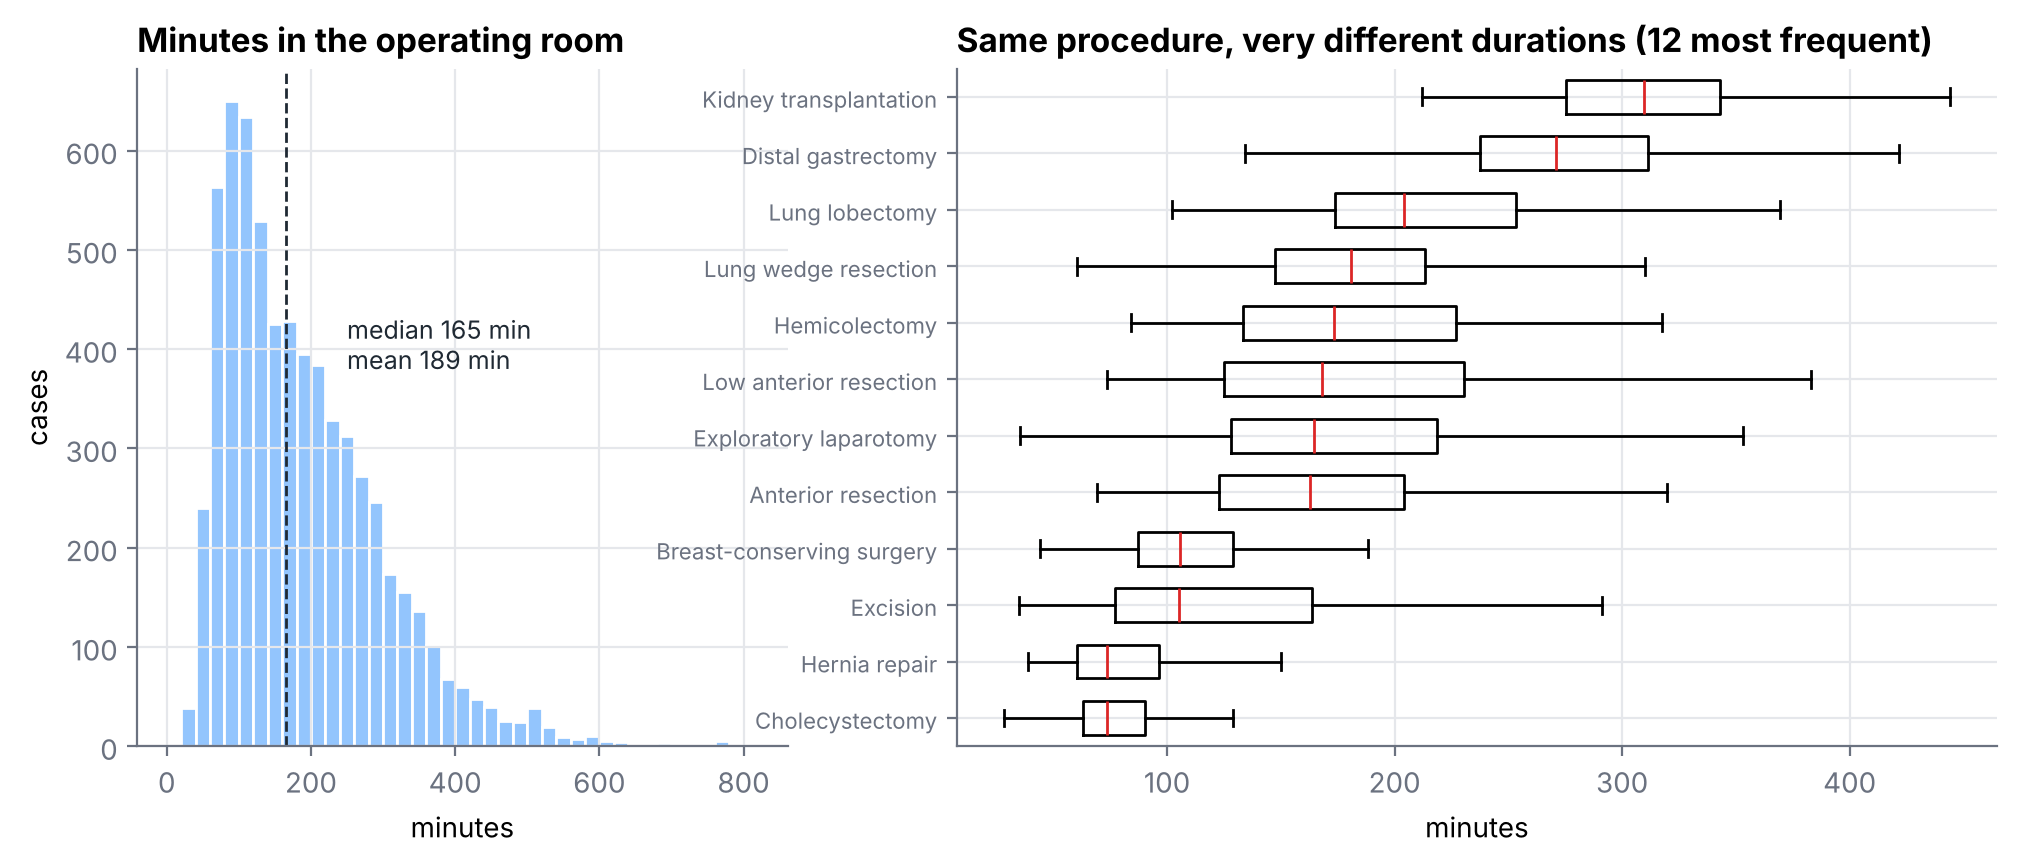
\includegraphics[width=\linewidth]{00_durations}
\caption{Distribution of case durations and variability within the twelve most frequent procedures.}\label{fig:eda}\end{figure}

\section{Methods}
\subsection{Point prediction}
Three predictors of the median duration are compared: the global training median (B0); the \emph{procedure history}
(B1), the median duration of the same procedure in the training set, falling back to the operation type and then to the
global median when fewer than ten past cases exist, which mimics common practice; and a histogram gradient-boosting model
(scikit-learn) trained with the pinball loss at level 0.5 (GBM), with native handling of categorical variables.

\subsection{Prediction intervals}
All intervals target a nominal coverage of $1-\alpha = 80\%$, i.e.\ the 10th to 90th percentiles.
\begin{description}
  \item[I1 Procedure history.] Empirical 10th and 90th percentiles of the same procedure (same fall-backs as B1).
  \item[I2 Quantile GBM.] Two gradient-boosting models trained with the pinball loss at 0.1 and 0.9 \cite{koenker1978}.
  \item[I3 Split conformal.] With $\hat m$ the GBM median, conformity scores $s_i=|\log y_i-\log\hat m(x_i)|$ are computed on
        the calibration set and $\hat k$ is their $\lceil (n+1)(1-\alpha)\rceil/n$ empirical quantile; the interval is
        $[\hat m e^{-\hat k},\ \hat m e^{\hat k}]$, a multiplicative band \cite{vovk2005,angelopoulos2021}.
  \item[I4 CQR.] Conformalized quantile regression \cite{romano2019}: with the quantile models $\hat q_{0.1},\hat q_{0.9}$,
        scores $s_i=\max(\hat q_{0.1}(x_i)-y_i,\ y_i-\hat q_{0.9}(x_i))$ give an adjustment $\hat k$ and the interval
        $[\hat q_{0.1}-\hat k,\ \hat q_{0.9}+\hat k]$, which keeps the case-specific width of quantile regression.
  \item[I5 CQR by department.] The same adjustment computed separately in each department (``Mondrian'' conformal
        prediction \cite{vovk2005}), to target coverage within departments rather than on average.
\end{description}
Split conformal methods guarantee marginal coverage of at least $1-\alpha$ when calibration and test cases are
exchangeable. Intervals are compared by coverage, mean width and the interval score
$W + \tfrac{2}{\alpha}(\ell-y)\mathbb{1}[y<\ell] + \tfrac{2}{\alpha}(y-u)\mathbb{1}[y>u]$ \cite{gneiting2007}, which rewards
narrow intervals and penalises misses (lower is better). Coverage is also reported by department, surgical approach and
tercile of predicted length. The whole evaluation is repeated on ten random patient-grouped splits; methods are compared
in pairs on the same splits.

\subsection{Scheduling under uncertainty}
A \emph{day} has $R=4$ identical operating rooms of capacity $C=480$ minutes and a waiting list of 24 elective cases
drawn at random from the test set. Let $m_i$ be the GBM median of case $i$. A planning rule decides which subsets of
cases may share a room:
\begin{itemize}
  \item \emph{historical}: $\sum_{i\in S} b_i \le C$ with $b_i$ the procedure-history median;
  \item \emph{ML median}: $\sum_{i\in S} m_i \le C$;
  \item \emph{fixed buffer} $\beta\in\{5,10,15,20,30\%\}$: $(1+\beta)\sum_{i\in S} m_i \le C$;
  \item \emph{quantile} $\tau\in\{0.6,0.7,0.8,0.9\}$: $\sum_{i\in S}\hat q_\tau(x_i)\le C$, with a quantile GBM per level;
  \item \emph{robust (learned set)} $\Gamma\in\{0.5,1,1.5,2,3\}$: $\sum_{i\in S} m_i + \max_{|T|\le\Gamma}\sum_{i\in T} d_i \le C$,
        the budget-of-uncertainty model of Bertsimas and Sim \cite{bertsimas2004}, where the deviations
        $d_i=u_i-m_i$ come from the conformal upper bound $u_i$ (I3), so that the uncertainty set is learned from data
        \cite{bertsimas2018}; a fractional $\Gamma$ counts that share of the next largest deviation.
\end{itemize}
Every rule then solves the same problem: choose at most $R$ disjoint feasible subsets maximising the planned workload
$\sum m_i$. Because rooms are identical, we enumerate all feasible subsets (a depth-first search with pruning, since
adding a case never decreases the load) and solve the set-packing model
\[
\max \sum_{S} \Big(\sum_{i\in S} m_i\Big) y_S \quad\text{s.t.}\quad \sum_{S\ni i} y_S\le 1\ \ \forall i,\qquad \sum_S y_S\le R,\qquad y_S\in\{0,1\}
\]
with HiGHS through SciPy. This pattern formulation is exact for every rule; a first, compact formulation of the robust
constraint with dual variables left optimality gaps of about 20\% within a 5-second limit and was abandoned. Each plan is
then evaluated with the \emph{real} durations: overtime $\max(0, L_r-C)$ and idle time $\max(0, C-L_r)$ per room, and
utilisation $\min(L_r,C)/C$. Results are averaged over 200 days; all rules see the same days, which allows paired
comparisons.

\section{Results}
\subsection{Point prediction}
\begin{table}[H]\centering\small
\begin{tabular}{lrrrr}\toprule
Model & MAE (min) & RMSE (min) & within $\pm$30 min & $R^2$ \\\midrule
B0 global median & 84.4 & 111.5 & 19.2\% & $-0.05$ \\
B1 procedure history & 48.3 & 71.9 & 48.8\% & 0.56 \\
GBM median & \textbf{43.9} & \textbf{65.2} & \textbf{51.1\%} & \textbf{0.64} \\\bottomrule
\end{tabular}
\caption{Point prediction on the test set (split 0). Over ten splits: GBM $45.6\pm1.3$ min, procedure history $50.7\pm1.8$ min.}
\end{table}
The procedure alone explains most of the predictable variation; patient and context variables add a 10\% reduction in
error. About half of the cases remain more than 30 minutes away from their prediction, which motivates intervals.

\subsection{Prediction intervals}
\begin{table}[H]\centering\small
\begin{tabular}{lrrrr}\toprule
Method & Coverage & Width (min) & Interval score & Worst department \\\midrule
I1 procedure history & $0.765\pm0.015$ & 146 & $241.7\pm8.6$ & 0.64 \\
I2 quantile GBM & $0.677\pm0.016$ & 123 & $238.7\pm7.5$ & 0.61 \\
I3 split conformal (log) & $0.805\pm0.010$ & 150 & $236.8\pm8.4$ & 0.77 \\
I4 CQR & $0.801\pm0.013$ & 148 & $\mathbf{231.5\pm6.6}$ & 0.74 \\
I5 CQR by department & $0.803\pm0.013$ & 150 & $231.9\pm6.4$ & 0.76 \\\bottomrule
\end{tabular}
\caption{80\% intervals, mean $\pm$ standard deviation over ten random splits. ``Worst department'': lowest coverage
among the four departments, averaged over splits.}\label{tab:int}
\end{table}
Both uncalibrated methods under-cover: the historical percentiles because a procedure's past cases do not represent
a new patient's uncertainty, the quantile GBM because quantiles fitted on the training set are too tight on new cases (67.7\% instead of 80\%). The two
conformal methods reach the target. Paired on the same splits, CQR has a lower interval score than the procedure
history in 10 of 10 splits (by $10.3\pm5.0$), than the quantile GBM in 10 of 10 ($7.3\pm1.7$) and than split
conformal in 9 of 10 ($5.4\pm4.9$): adapting the width to each case pays off.

\begin{figure}[H]\centering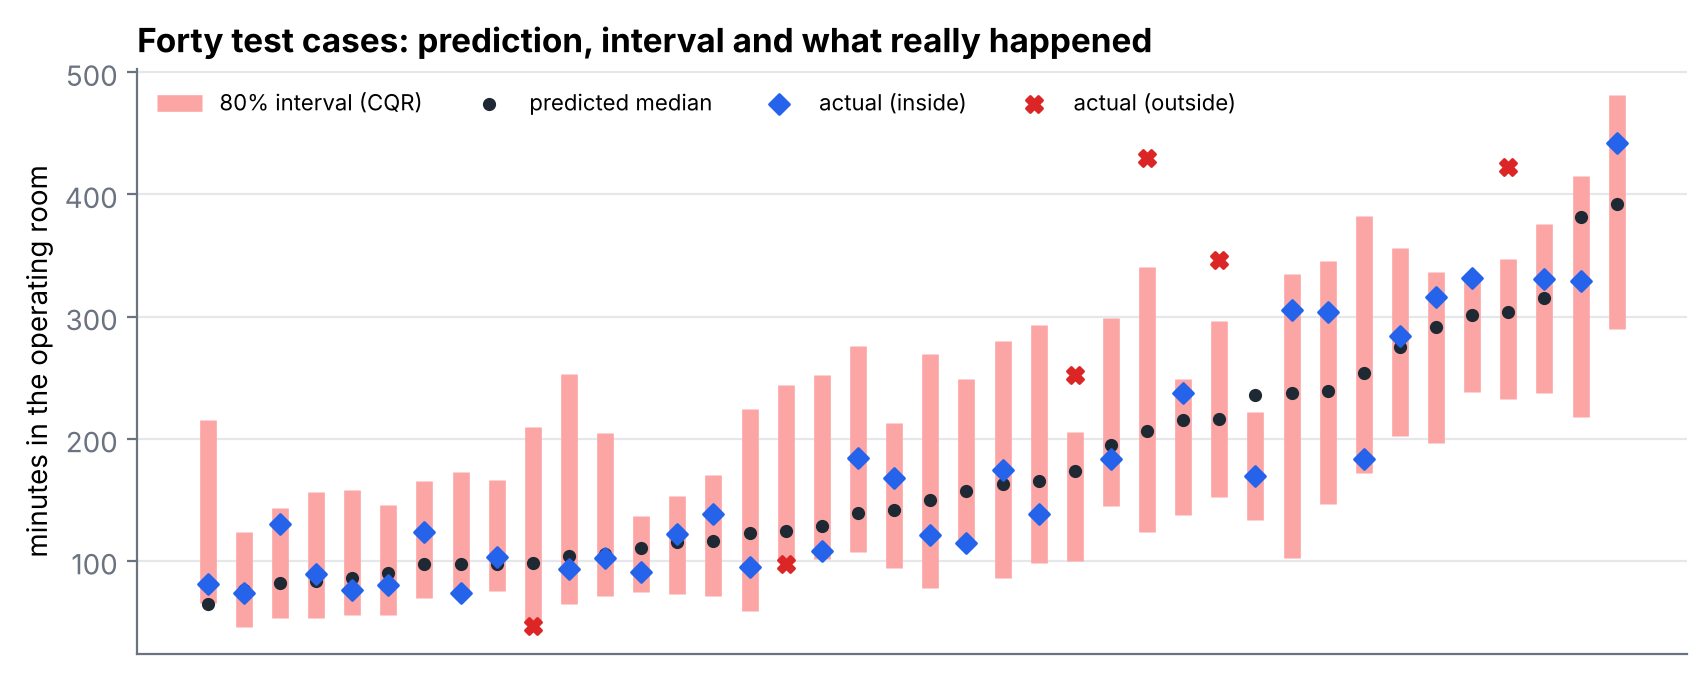
\includegraphics[width=\linewidth]{01_intervals_examples}
\caption{Forty test cases with their median prediction, CQR interval and actual duration.}\end{figure}
\begin{figure}[H]\centering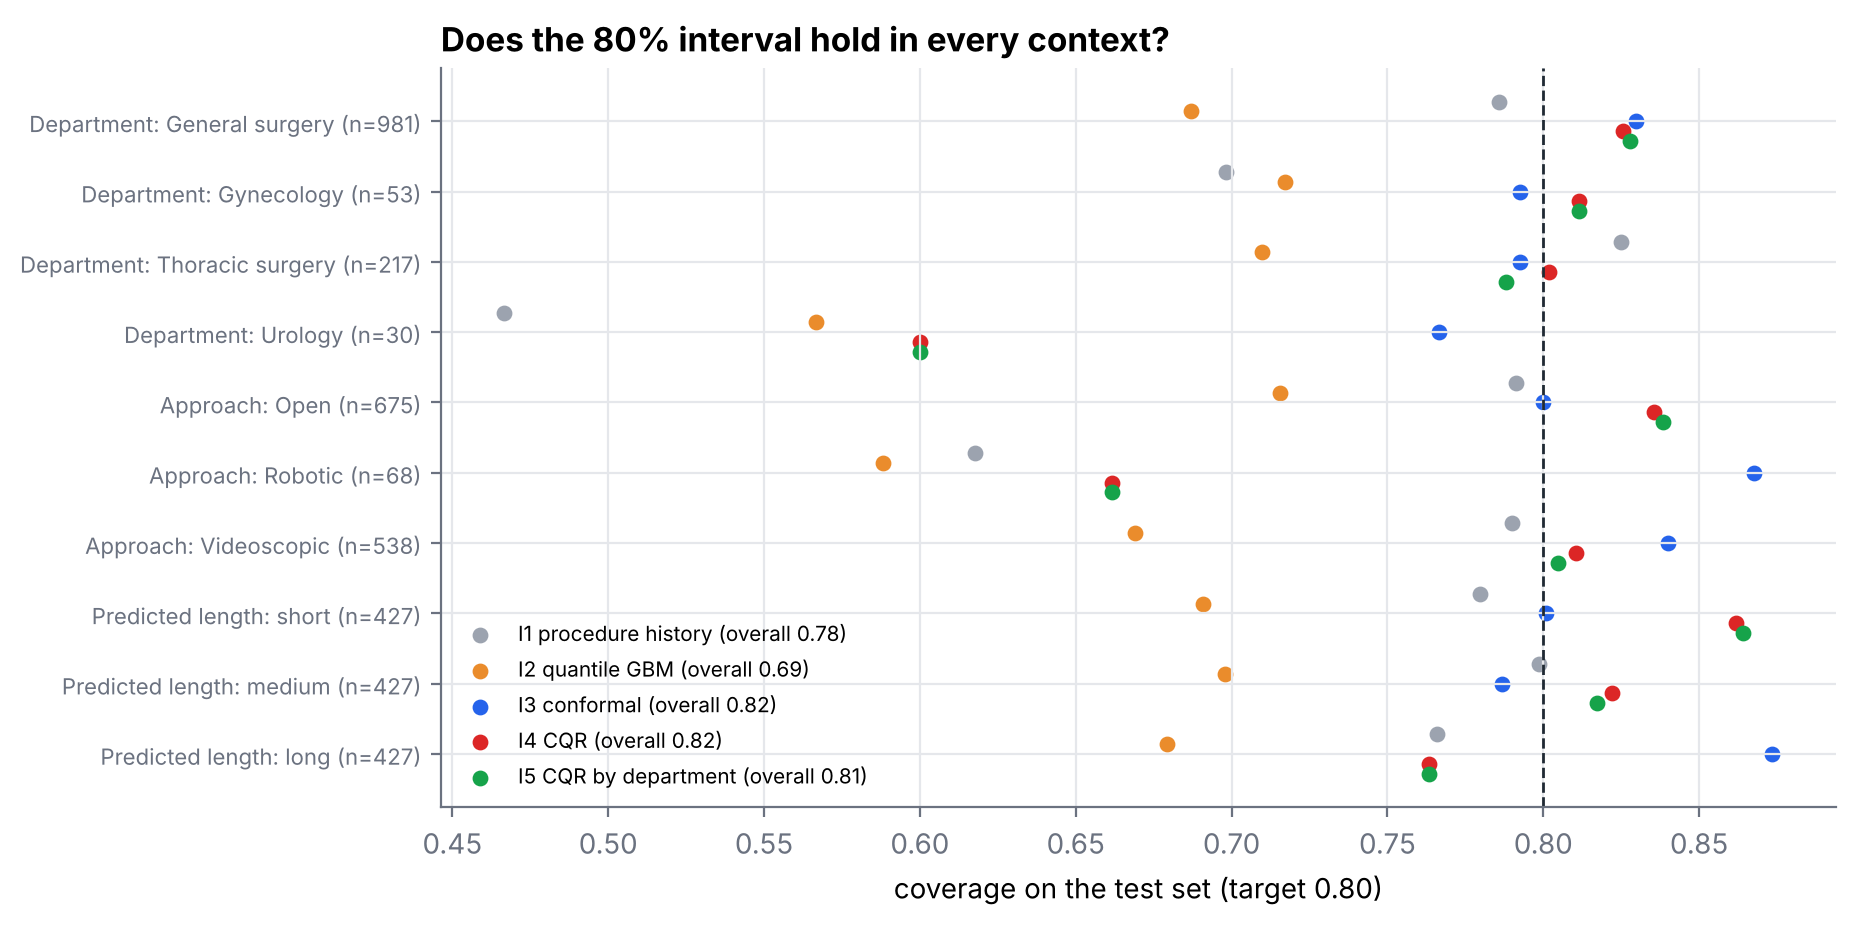
\includegraphics[width=0.85\linewidth]{02_coverage}
\caption{Coverage by surgical context on the test set of split 0.}\label{fig:cov}\end{figure}

Marginal coverage hides differences between contexts (Figure~\ref{fig:cov}). With CQR, coverage is 0.66 for robotic
surgery ($n=68$) and 0.60 in urology ($n=30$), while the long-case tercile is slightly under-covered (0.76). Small groups
are noisy, but the pattern is consistent: rare contexts are under-represented in the calibration set. Calibrating per
department (I5) raises the worst department's coverage on average (0.74 to 0.76) at almost no cost in score
($+0.4\pm0.5$), but cannot fix urology, which has only about 20 calibration cases. The log-scale conformal band (I3), whose
width grows with the prediction, behaves best for long cases and the robotic approach.

\subsection{Effect on schedules}
\begin{figure}[H]\centering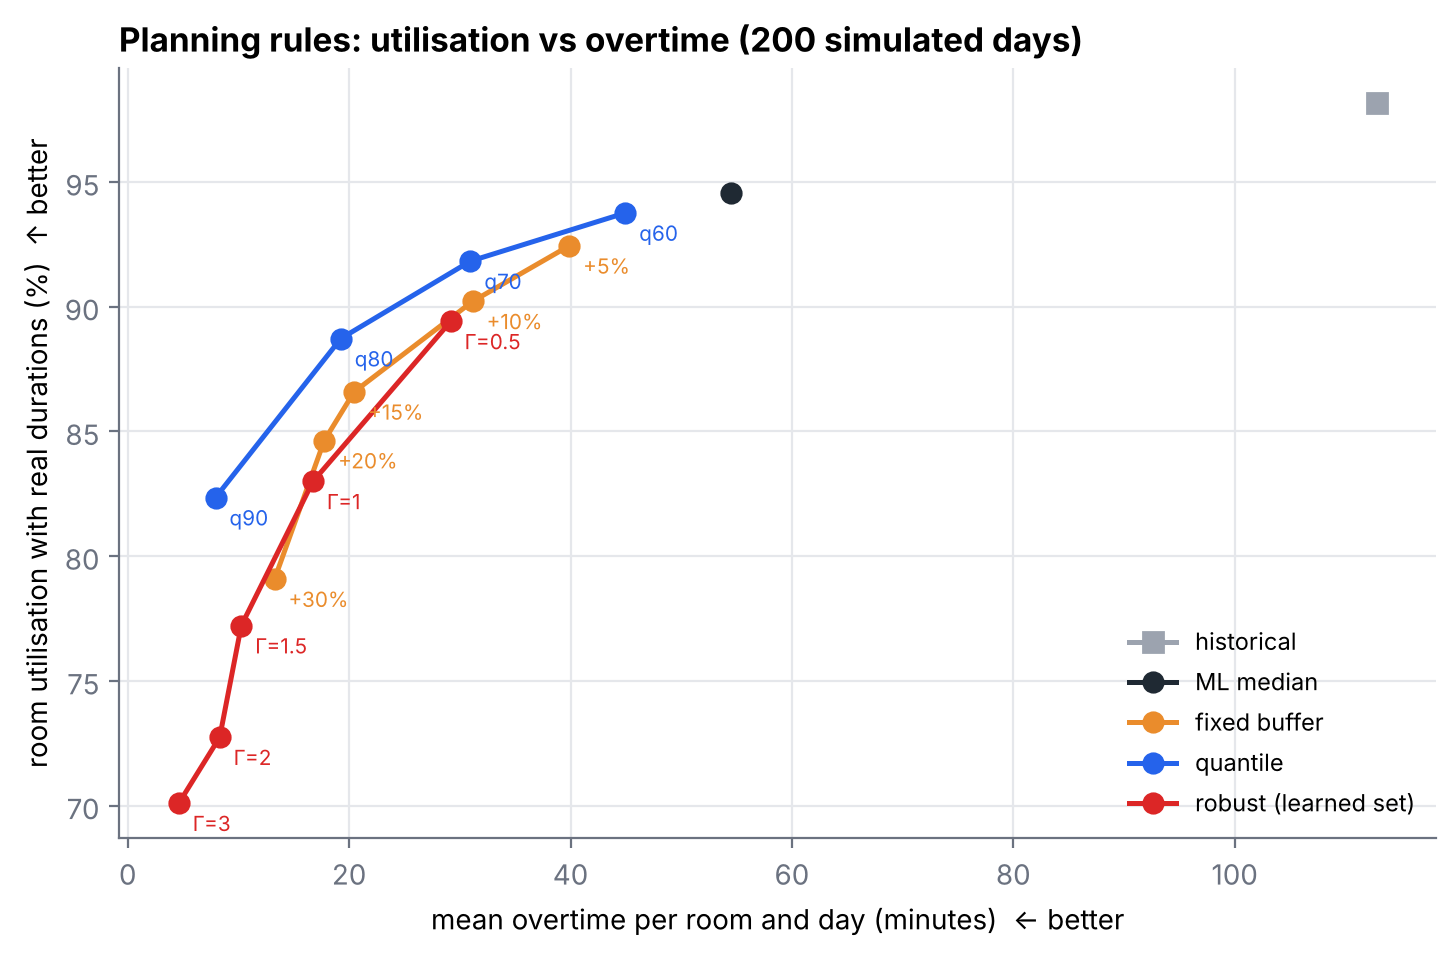
\includegraphics[width=0.85\linewidth]{03_schedule_frontier}
\caption{Utilisation against overtime for each planning rule (200 simulated days; each point is one parameter value).}\label{fig:front}\end{figure}

\begin{table}[H]\centering\small
\begin{tabular}{lrrrr}\toprule
Rule & Overtime (min/room/day) & Rooms in overtime & Utilisation & Cases/day \\\midrule
historical medians & 112.8 & 79.6\% & 98.2\% & 12.5 \\
ML median & 54.5 & 55.4\% & 94.6\% & 12.6 \\
fixed buffer +15\% & 20.5 & 26.8\% & 86.6\% & 11.2 \\
quantile $\tau=0.8$ & 19.2 & 29.5\% & 88.7\% & 9.3 \\
fixed buffer +30\% & 13.3 & 16.0\% & 79.1\% & 10.2 \\
quantile $\tau=0.9$ & 7.9 & 15.4\% & 82.3\% & 7.8 \\
robust $\Gamma=2$ & 8.3 & 10.2\% & 72.7\% & 10.7 \\\bottomrule
\end{tabular}
\caption{Selected planning rules (all rules in \texttt{results/schedule\_summary.csv}).}\label{tab:sched}
\end{table}

Planning on medians systematically overruns: durations are right-skewed, so each case's real duration exceeds its
predicted median by 10.4 minutes on average, and these excesses add up within a room. With the less precise historical
medians, 80\% of rooms finish late. The learned per-case quantiles dominate the other rules over the whole range
(Figure~\ref{fig:front}). At about 20 minutes of overtime, the 80th percentile keeps 2.1 points more utilisation than a
uniform 15\% buffer ($\pm1.1$, paired 95\% interval). At about 8 minutes of overtime, the 90th percentile keeps 9.6 points
more utilisation than the robust model with $\Gamma=2$ ($\pm1.3$), and against a 30\% buffer it gains 3.3 points while
cutting overtime by 5.3 minutes. Per-case quantiles place the safety margin where the uncertainty is, whereas a uniform
buffer protects short, predictable cases as much as long, uncertain ones.

The budgeted robust model was the most conservative: it protects every room against its $\Gamma$ largest deviations
simultaneously, a worst case that rarely happens, and conformal upper bounds are wide (they cover 90\% of cases on their
own). It also schedules more, shorter cases, which explains its high case count with low utilisation. A
distributionally robust or chance-constrained model that accounts for partial compensation between cases in a room would
be the natural next step. Finally, we checked whether the optimiser favours cases whose duration is underestimated (the
``optimiser's curse''): under the ML-median rule, scheduled cases exceed their prediction by 9.3 minutes on average,
close to the 10.4 minutes of all elective cases, so the effect is not visible here.

\section{Limitations}
\begin{itemize}
  \item \textbf{One hospital, no dates.} VitalDB comes from a single Korean centre; results may not transfer, and the
        random split ignores changes over time (new surgeons, techniques).
  \item \textbf{No recovery room.} VitalDB has no PACU timestamps, so downstream capacity, central in practice
        \cite{shehadeh2022}, is not modelled.
  \item \textbf{Simplified schedules.} Identical rooms, no surgeon or equipment constraints, no sequencing within a
        room, no emergencies; the waiting list is drawn at random.
  \item \textbf{Exchangeability.} Conformal guarantees are marginal and assume that new cases resemble the calibration
        cases; they do not hold within small groups.
\end{itemize}

\section{Conclusion}
On open data, the uncertainty of surgery duration can be learned and calibrated: conformalized quantile regression
gives honest 80\% intervals that are narrower where cases are predictable. Used directly as planning durations, these
learned quantiles give better schedules than historical averages or uniform buffers, with less overtime for the same
utilisation. Making coverage hold in every surgical context, and combining learned uncertainty with downstream
recovery-room capacity, are the two directions this study leaves open.

\paragraph{Reproducibility.} \texttt{python run\_all.py} downloads VitalDB and regenerates every number and figure
(about ten minutes on a laptop). A sample of cases exported as HL7 FHIR R4 Patient, Encounter and Procedure resources is
included as a first step towards a reusable data pipeline.

\begin{thebibliography}{99}\small
\bibitem{angelopoulos2021} A.~N. Angelopoulos, S.~Bates. A gentle introduction to conformal prediction and
  distribution-free uncertainty quantification. arXiv:2107.07511, 2021.
\bibitem{bertsimas2004} D.~Bertsimas, M.~Sim. The price of robustness. \emph{Operations Research}, 52(1):35--53, 2004.
\bibitem{bertsimas2018} D.~Bertsimas, V.~Gupta, N.~Kallus. Data-driven robust optimization. \emph{Mathematical
  Programming}, 167(2):235--292, 2018.
\bibitem{cardoen2010} B.~Cardoen, E.~Demeulemeester, J.~Beliën. Operating room planning and scheduling: a literature
  review. \emph{European Journal of Operational Research}, 201(3):921--932, 2010.
\bibitem{gneiting2007} T.~Gneiting, A.~E. Raftery. Strictly proper scoring rules, prediction, and estimation.
  \emph{Journal of the American Statistical Association}, 102(477):359--378, 2007.
\bibitem{koenker1978} R.~Koenker, G.~Bassett. Regression quantiles. \emph{Econometrica}, 46(1):33--50, 1978.
\bibitem{martinez2021} O.~Martinez, C.~Martinez, C.~A. Parra, S.~Rugeles, D.~R. Suarez. Machine learning for surgical
  time prediction. \emph{Computer Methods and Programs in Biomedicine}, 208:106220, 2021.
\bibitem{romano2019} Y.~Romano, E.~Patterson, E.~Candès. Conformalized quantile regression. \emph{Advances in Neural
  Information Processing Systems 32}, 2019.
\bibitem{shehadeh2022} K.~S. Shehadeh, R.~Padman. Stochastic optimization approaches for elective surgery scheduling
  with downstream capacity constraints: models, challenges, and opportunities. \emph{Computers \& Operations Research},
  137:105523, 2022.
\bibitem{vitaldb} H.-C. Lee, Y.~Park, S.~B. Yoon, S.~M. Yang, D.~Park, C.-W. Jung. VitalDB, a high-fidelity
  multi-parameter vital signs database in surgical patients. \emph{Scientific Data}, 9:279, 2022.
\bibitem{vovk2005} V.~Vovk, A.~Gammerman, G.~Shafer. \emph{Algorithmic Learning in a Random World}. Springer, 2005.
\end{thebibliography}
\end{document}
